\documentclass[12pt]{article}
\usepackage[margin=1in]{geometry} 
\usepackage{amsmath,amsthm,amssymb,amsfonts}
\usepackage{graphicx}

\newcommand{\N}{\mathbb{N}}
\newcommand{\Z}{\mathbb{Z}}
 
\newenvironment{problem}[2][Problem]{\begin{trivlist}
\item[\hskip \labelsep {\bfseries #1}\hskip \labelsep {\bfseries #2.}]}{\end{trivlist}}
 
\begin{document}
 
\title{Math 451 - H1}
\author{Lucas Wilson}
\maketitle
 
\begin{problem}{1}
\end{problem}

\begin{tabular}{ c | c | c | c | c | c }
n & time (s) & det(A) & actual det(A) & error & relative error \\
\hline
1 & 0.00 & 1.00000e+00 & 1.00000e+00 & 0.00000e+00 & 0.00000e+00 \\
2 & 0.00 & -2.67949e-01 & -2.67949e-01 & 1.66533e-16 & -6.21511e-16 \\
3 & 0.00 & 2.65394e-03 & 2.65394e-03 & -6.06720e-16 & -2.28611e-13 \\
4 & 0.00 & -1.41317e-06 & -1.41317e-06 & -1.30008e-16 & 9.19978e-11 \\
5 & 0.00 & 4.37205e-11 & 4.37204e-11 & -6.33895e-17 & -1.44988e-06 \\
6 & 0.00 & -8.11334e-17 & -8.09559e-17 & 1.77473e-19 & -2.19222e-03 \\
7 & 0.01 & -1.77904e-21 & 9.10361e-24 & 1.78814e-21 & 1.96422e+02 \\
8 & 0.13 & 2.68053e-25 & -6.26851e-32 & -2.68053e-25 & 4.27619e+06 \\
9 & 1.12 & 2.65011e-29 & 2.65669e-41 & -2.65011e-29 & -9.97523e+11 \\
10 & 11.14 & -7.48538e-34 & -6.94248e-52 & 7.48538e-34 & -1.07820e+18 \\
11 & 135.20 & 9.45310e-40 & 9.78267e-64 & -9.45310e-40 & -9.66311e+23 \\
\end{tabular}
\newline
\newline
Notice that after n=6, relative error starts to grow. This is due to perturbation of error at a rate of $n!$ since the algorithm is $O(n!)$. After $n=10$, the algorithm takes too long to calculate, 2 minutes. Post $n=11$, it will probably be $2*12=24$ minutes.
\\

\begin{problem}{2}
\end{problem}

\begin{tabular}{ c | c | c | c | c | c }
n & time (s) & det(A) & actual det(A) & error & relative error \\
\hline
1 & 0.00 & 1.00000e+00 & 1.00000e+00 & 0.00000e+00 & 0.00000e+00 \\
2 & 0.00 & -2.67949e-01 & -2.67949e-01 & 1.66533e-16 & -6.21511e-16 \\
3 & 0.00 & 2.65394e-03 & 2.65394e-03 & 7.19910e-17 & 2.71261e-14 \\
4 & 0.00 & -1.41317e-06 & -1.41317e-06 & -3.47728e-18 & 2.46063e-12 \\
5 & 0.00 & 4.37204e-11 & 4.37204e-11 & 1.56932e-22 & 3.58944e-12 \\
6 & 0.00 & -8.09559e-17 & -8.09559e-17 & 6.62940e-26 & -8.18890e-10 \\
7 & 0.00 & 9.10361e-24 & 9.10361e-24 & 5.27834e-32 & 5.79807e-09 \\
8 & 0.00 & -6.26851e-32 & -6.26851e-32 & -3.42316e-38 & 5.46089e-07 \\
9 & 0.00 & 2.65672e-41 & 2.65669e-41 & -3.09812e-46 & -1.16616e-05 \\
10 & 0.00 & -6.95205e-52 & -6.94248e-52 & 9.57062e-55 & -1.37856e-03 \\
\end{tabular}
\newline
\newline
\begin{tabular}{ c | c | c | c | c | c }
n & time (s) & det(A) & actual det(A) & error & relative error \\
\hline
11 & 0.00 & 9.55886e-64 & 9.78267e-64 & 2.23814e-65 & 2.28786e-02 \\
12 & 0.00 & 1.02658e-75 & 8.39606e-76 & -1.86977e-76 & -2.22696e-01 \\
13 & 0.00 & -3.73159e-88 & -5.15872e-88 & -1.42712e-88 & 2.76643e-01 \\
14 & 0.00 & 2.56800e-101 & 1.12709e-100 & 8.70293e-101 & 7.72157e-01 \\
15 & 0.00 & 1.97241e-113 & 3.12162e-113 & 1.14921e-113 & 3.68145e-01 \\
16 & 0.00 & -4.19287e-126 & -1.90027e-126 & 2.29260e-126 & -1.20646e+00 \\
17 & 0.00 & 2.99048e-139 & 3.65475e-140 & -2.62501e-139 & -7.18246e+00 \\
18 & 0.00 & -6.40505e-152 & -8.75399e-154 & 6.31751e-152 & -7.21672e+01 \\
19 & 0.00 & 2.03723e-164 & -1.02402e-165 & -2.13963e-164 & 2.08944e+01 \\
20 & 0.01 & -3.40696e-177 & 3.30948e-179 & 3.44005e-177 & 1.03945e+02 \\
21 & 0.01 & 1.76273e-189 & 8.09643e-192 & -1.75463e-189 & -2.16717e+02 \\
22 & 0.01 & -2.26503e-202 & -9.15550e-205 & 2.25588e-202 & -2.46396e+02 \\
23 & 0.01 & 9.70105e-216 & -5.49439e-219 & -9.70654e-216 & 1.76663e+03 \\
24 & 0.01 & 1.50532e-228 & -1.40645e-231 & -1.50673e-228 & 1.07130e+03 \\
25 & 0.01 & -1.01324e-241 & -7.26910e-246 & 1.01317e-241 & -1.39380e+04 \\
26 & 0.01 & -1.35169e-254 & 1.53119e-258 & 1.35185e-254 & 8.82873e+03 \\
27 & 0.01 & -2.88297e-268 & -1.17796e-273 & 2.88295e-268 & -2.44742e+05 \\
28 & 0.01 & 2.06971e-281 & 4.80717e-286 & -2.06966e-281 & -4.30537e+04 \\
29 & 0.01 & -1.20034e-293 & 2.61847e-298 & 1.20036e-293 & 4.58421e+04 \\
30 & 0.01 & 1.60391e-306 & -1.91678e-312 & -1.60391e-306 & 8.36773e+05 \\
31 & 0.01 & -6.27414e-320 & 0.00000e+00 & 6.27414e-320 & inf \\
32 & 0.01 & 0.00000e+00 & -0.00000e+00 & -0.00000e+00 & nan \\
33 & 0.01 & 0.00000e+00 & 0.00000e+00 & 0.00000e+00 & nan \\
34 & 0.02 & 0.00000e+00 & -0.00000e+00 & -0.00000e+00 & nan \\
35 & 0.02 & -0.00000e+00 & 0.00000e+00 & 0.00000e+00 & nan \\
36 & 0.02 & 0.00000e+00 & 0.00000e+00 & 0.00000e+00 & nan \\
37 & 0.02 & 0.00000e+00 & -0.00000e+00 & -0.00000e+00 & nan \\
38 & 0.02 & -0.00000e+00 & 0.00000e+00 & 0.00000e+00 & nan \\
39 & 0.02 & -0.00000e+00 & 0.00000e+00 & 0.00000e+00 & nan \\
40 & 0.02 & -0.00000e+00 & 0.00000e+00 & 0.00000e+00 & nan \\
41 & 0.02 & -0.00000e+00 & -0.00000e+00 & 0.00000e+00 & nan \\
42 & 0.02 & -0.00000e+00 & -0.00000e+00 & 0.00000e+00 & nan \\
43 & 0.02 & 0.00000e+00 & 0.00000e+00 & 0.00000e+00 & nan \\
44 & 0.03 & 0.00000e+00 & -0.00000e+00 & -0.00000e+00 & nan \\
45 & 0.03 & 0.00000e+00 & -0.00000e+00 & -0.00000e+00 & nan \\
46 & 0.03 & -0.00000e+00 & -0.00000e+00 & 0.00000e+00 & nan \\
47 & 0.03 & 0.00000e+00 & -0.00000e+00 & -0.00000e+00 & nan \\
48 & 0.03 & 0.00000e+00 & -0.00000e+00 & -0.00000e+00 & nan \\
49 & 0.04 & -0.00000e+00 & 0.00000e+00 & 0.00000e+00 & nan \\
50 & 0.03 & -0.00000e+00 & 0.00000e+00 & 0.00000e+00 & nan \\
\end{tabular}
\newline
\newline
\begin{tabular}{ c | c | c | c | c | c }
n & time (s) & det(A) & actual det(A) & error & relative error \\
\hline
100 & 0.13 & -0.00000e+00 & -0.00000e+00 & 0.00000e+00 & nan \\
150 & 0.31 & -0.00000e+00 & 0.00000e+00 & 0.00000e+00 & nan \\
200 & 0.54 & 0.00000e+00 & 0.00000e+00 & 0.00000e+00 & nan \\
250 & 0.84 & -0.00000e+00 & -0.00000e+00 & 0.00000e+00 & nan \\
300 & 1.25 & 0.00000e+00 & 0.00000e+00 & 0.00000e+00 & nan \\
350 & 1.68 & 0.00000e+00 & 0.00000e+00 & 0.00000e+00 & nan \\
400 & 2.19 & -0.00000e+00 & 0.00000e+00 & 0.00000e+00 & nan \\
450 & 2.85 & 0.00000e+00 & -0.00000e+00 & -0.00000e+00 & nan \\
500 & 3.56 & 0.00000e+00 & 0.00000e+00 & 0.00000e+00 & nan \\
600 & 10.65 & 0.00000e+00 & 0.00000e+00 & 0.00000e+00 & nan \\
700 & 7.21 & 0.00000e+00 & -0.00000e+00 & -0.00000e+00 & nan \\
800 & 9.37 & -0.00000e+00 & -0.00000e+00 & 0.00000e+00 & nan \\
900 & 12.54 & -0.00000e+00 & -0.00000e+00 & 0.00000e+00 & nan \\
1000 & 16.22 & 0.00000e+00 & 0.00000e+00 & 0.00000e+00 & nan \\
1250 & 26.66 & -0.00000e+00 & -0.00000e+00 & 0.00000e+00 & nan \\
1500 & 74.80 & 0.00000e+00 & -0.00000e+00 & -0.00000e+00 & nan \\
\end{tabular}
\newline
\newline

$n$ can be significantly larger than before. This has to do with the algorithm now
being $O(n^3)$, but the matrix is so large the determinant is zero.
\\

\begin{problem}{3}
\end{problem}

In the graph, I made the y-axis smaller so that the zeros are easier to see. I made the x-axis large enough to include all zeros. That, however, makes it difficult to see grouped zeros.
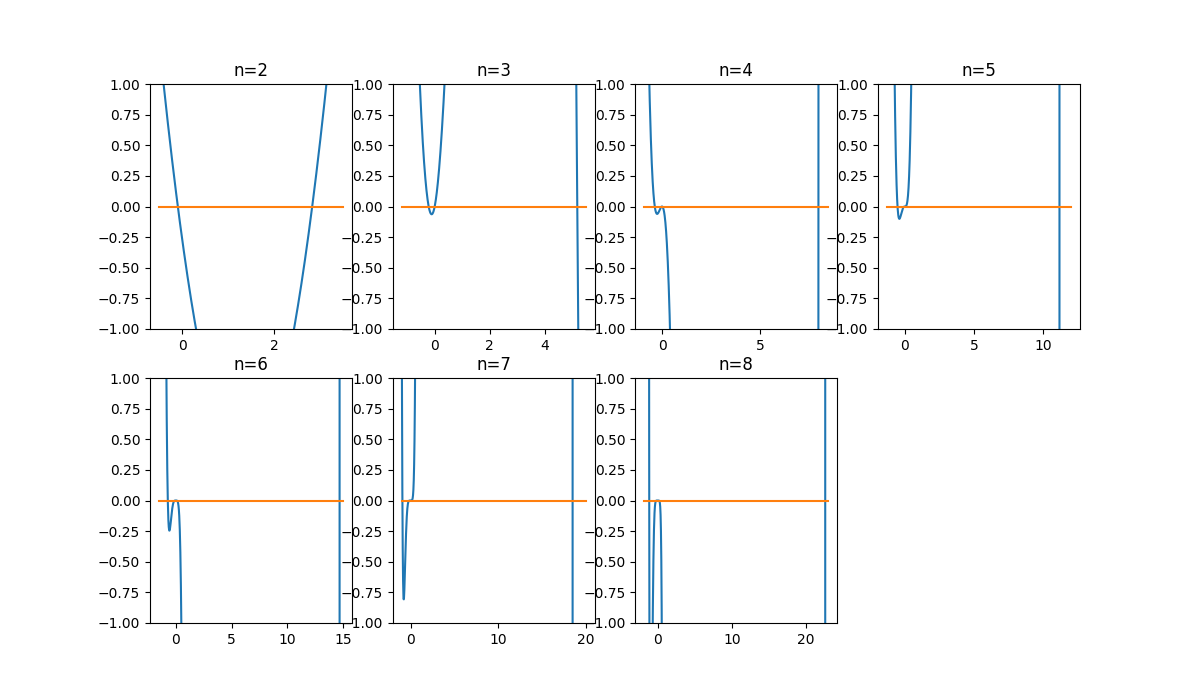
\includegraphics[width=\textwidth]{p3.png}

\noindent
Estimated eigenvalues:
\\
For $n=2, \lambda = -0.091033, 2.82235$ \\
For $n=3, \lambda = -.209392, 0.00911226, 5.21679$ \\
For $n=4, \lambda = -0.358778, 0.0499652 ($mul$: 2), 8.02046$ \\
For $n=5, \lambda = -0.505941, 0.0723875 ($mul$: 3), 11.2052$ \\
For $n=6, \lambda = -0.620171, 0.0076199 ($mul$: 4), 14.7159$ \\
For $n=7, \lambda = -0.92237, -0.18424 ($mul$: 5), 18.5416$ \\
For $n=8, \lambda = -1.18027, 0.169067 ($mul$: 6), 22.7029$ \\

\noindent
Verification:
\\
For $n=2$
\\
$
(1-\lambda)(\sqrt3-\lambda)-2
\\
\lambda^2-(1+\sqrt3)\lambda+\sqrt3-2
\\
$
Using quadratic formula..
$\lambda = 2.82684, -0.0947876$
\\
For $n=3$
\\
$(1-\lambda)((\sqrt3-\lambda)(\sqrt5-\lambda)-4)-\sqrt2((\sqrt2(\sqrt5-\lambda))-\sqrt12)+\sqrt3(\sqrt8-\sqrt3(\sqrt3-\lambda))$
\\
Using the cubic formula.. (aka Wolfram Alpha)
\\
$\lambda = 5.19145, -0.221018, -0.002313$
\\
All these eigenvalues were fairly accurately approximated.
\\

\begin{problem}{4}
\end{problem}

From the previous problem, we can find where all the eigenvalues should be, roughly. Then we can use methods like Newton's method, secant method, or bisection method to solve for the exact zeros. I'll choose secant method. Bisection won't work for zeros with an even multiplicity, and Newton's method requires taking derivatives.
\\

The formula and error for secant method is as follows:
\\

$x_{n+1}=\frac{f(x_n)x_{n-1} - f(x_{n-1})x_n}{f(x_n)-f(x_{n-1})}$, where $f(x)=det(A-xI)$
\\

$e_n=e_n e_{n-1}=e_{n-1}^{\phi}$, where $\phi = \frac{1+\sqrt5}{2}$
\\

$x_n$ is a sequence which converges to the real value of $\lambda$ since $f(x)$ equals the characteristic polynomial. $e_n$ is the error. Since we do not know the initial error, we can give it an upper bound instead. When we chose our initial guess for $\lambda$, we can assume it's at most $0.5$ away from its actual value: $e_0=0.5$. The only requirement is that $e_0<1$ or else $e_n$ won't converge.

$e_0<1\implies e_n \to 0$, so you can find an n such that $n>N \implies |e_n|<\epsilon$. Then, you know that your $\lambda$ is within $\epsilon$ of the real $\lambda$.
\\

Complexity:
\\

In calculating the next iteration of $\lambda$, the complexity is 1 new evaluation of $f(x_n)$, 2 multiplications, 2 subtractions and 1 division. The 5 operations are drowned in the complexity of calculating $f(x_n)$, the next approximation for $\lambda$, which is the complexity of Problem 2, $O(n^3)$.
\\

Now, the number of iterations needs to be considered. We are trying to find an $N$ such that $e_0^{N\phi}<\epsilon$.
\\

$e_0^{N\phi}<\epsilon \implies N = \log_{e_0^\phi} \epsilon$
Since we need to perform N iterations, the complexity is
\\

$O(N n^3)=O(n^3 \log_{e_0^\phi} \epsilon)$
\\

where $e_0$ is the initial upper bound for error (a reasonable value is $0.5$) and $\phi = \frac{1+\sqrt5}{2}$.

\begin{problem}{5}
\end{problem}

Tridiagonal
$
A_n=
  \left[ {\begin{array}{cccccc}
  a_{11} & a_{12} & 0 & 0 & ... & 0 \\
  a_{21} & a_{22} & a_{23} & 0 \\
  0 & a_{32} & a_{33} & a_{34} & & ... \\
  0 & 0 & a_{43} & a_{44} \\
  ... & & & & ... \\
  0 & ... & & 0 & a_{n-1,n}& a_{nn}
  \end{array} } \right]
$
\\

Algorithm 1:
\\

Each row is processed. The first element in the row is noted and the row and column are removed, leaving a smaller matrix. This constant is multiplied by the determinant of the smaller matrix and contributes to the sum. Thus, it is 1 multiplication and the determinant of a smaller matrix.
\\

For the first row, this smaller matrix takes the same form, so the complexity is n for the first rows. For the second row, the smaller matrix takes the same form except $a_{21}=0$. Thus, the complexity is n for the second rows as well. Thus, the overall complexity of Problem 1's algorithm is $O(2^n)$.
\\

Algorithm 2:
\\

For this algorithm, the elements below the main diagonal need to be zeroed out. They are zeroed from top left to right by adding a multiple of the row before it. There are $n-1$ of these rows with $n/2$ elements on average; thus, $O(n^2)$ elements in total, so $O(n^2)$ multiplications. There is an additional n multiplications of the diagonal elements for calculating the determinant, but $O(n)$ is a lower order than $O(n^2)$. Thus, the complexity for Problem 2's algorithm is $O(n^2)$
\\

Analysis
\\
In both cases, the algorithms' complexity is independent of the upper parts of the matrix. Thus the difference between tridiagonal and Hessenberg don't matter with respect to complexity.

\end{document}
